\chapter{Módulo: Clínica}
\label{mod:05-clinica}

\section{Propósito}
\label{sec:clinica-proposito}

Registra la historia clínica de cada paciente (consultas) y la receta óptica resultante, con generación de PDF y acceso propio del paciente a su historial y recetas desde el portal. Una receta puede nacer de una consulta o cargarse manualmente sin consulta previa (``externa''), para cubrir el caso de un cliente que trae una receta de otra óptica.

\section{Entidades principales}
\label{sec:clinica-entidades}

\begin{longtable}{p{3.0cm}p{10.3cm}}
\caption{Entidades principales del módulo de Clínica.}\label{tab:clinica-entidades}\\
\toprule
\textbf{Entidad} & \textbf{Rol} \\
\midrule
\endfirsthead
\toprule
\textbf{Entidad} & \textbf{Rol} \\
\midrule
\endhead
\bottomrule
\endfoot
\code{ConsultaClinica} & Cabecera de la consulta: paciente, profesional, sucursal, motivo, diagnóstico. Ver Capítulo~\ref{sec:modelo-datos}, Grupo B. \\
\code{Receta} & Graduación óptica (OD/OI: esférico, cilindro, eje, adición), 1:1 opcional con una consulta \textbf{o} vinculada directo a una \code{Person} (externa). Ver Capítulo~\ref{sec:modelo-datos}, Grupo B. \\
\end{longtable}

\section{Reglas de negocio clave}
\label{sec:clinica-reglas}

\begin{itemize}
  \item \textbf{El profesional se autoasigna desde el JWT} (claim \code{professional_id}), nunca se selecciona en el formulario: al crear/editar una consulta, si quien llama es un profesional, el backend sobrescribe \code{ProfessionalId} con el propio, ignorando lo que venga en el request. El listado (\code{GET /api/consultas}) también se auto-filtra a las consultas del profesional autenticado.
  \item \textbf{Receta clínica o externa} --- ver \hyperref[adr:0008]{ADR 0008}: una \code{Receta} puede colgar de una \code{ConsultaClinica} (1:1, \code{Cascade}) o cargarse manual para una \code{Person} sin consulta (\code{PersonId}, sin \code{ConsultaClinicaId}). El flujo de venta a pedido consume ambas por igual vía \code{GET /api/recetas?clienteId=}.
  \item \textbf{El estado de una consulta NO es un enum C\#, a diferencia de \code{Turno}.} \code{ConsultaClinica} no tiene columna \code{Estado}: su único campo de estado es \code{EstadoConfigId} (FK a \code{EstadoConfig}, la misma tabla de configuración que en \code{Turno} es puramente cosmética --- ver Capítulo~\ref{mod:04-agenda-turnos}). Para Consulta, en cambio, \code{EstadoConfig} \textbf{sí es funcional}: \code{ConsultaClinicaService.}\allowbreak \code{CreateAsync} busca la fila con \code{Entidad == "Consulta" && CodigoInterno == "Abierta"} para asignar el estado inicial. Los 4 estados reales (verificados en \code{DbSeeder.}\allowbreak \code{EstadosIniciales}) son \textbf{Pendiente, Abierta, Cerrada, Cancelada}.
  \item \textbf{PDF de receta} (\code{QuestPDF}, A5, 1.5cm de margen): \code{GET /api/consultas/{id}/receta/pdf} devuelve 404 si la consulta no tiene receta cargada. El paciente tiene su propio endpoint equivalente (\code{/mi-receta/pdf}) que valida que la consulta le pertenezca antes de generar el archivo.
  \item \textbf{Portal del paciente de solo lectura:} \code{mis-consultas} y \code{mi-receta/pdf} resuelven el \code{patientId} a partir del \code{userId} del JWT (el JWT no trae \code{patient_id} directo), replicando el mismo patrón de resolución que usa \code{TurnoService}.
\end{itemize}

\section{Endpoints}
\label{sec:clinica-endpoints}

\begin{longtable}{p{3.5cm}p{4cm}p{6cm}}
\caption{Endpoints principales del módulo de Clínica.}\label{tab:clinica-endpoints}\\
\toprule
\textbf{Método} & \textbf{Ruta} & \textbf{Descripción} \\
\midrule
\endfirsthead
\toprule
\textbf{Método} & \textbf{Ruta} & \textbf{Descripción} \\
\midrule
\endhead
\bottomrule
\endfoot
GET & \code{/api/consultas} & Listado paginado (auto-filtrado si el caller es profesional) \\
GET & \code{/}\allowbreak \code{api/}\allowbreak \code{consultas/}\allowbreak \code{{id}} $\cdot$ \code{/}\allowbreak \code{patient/}\allowbreak \code{{patientId}} & Detalle / por paciente \\
GET & \code{/}\allowbreak \code{api/}\allowbreak \code{consultas/}\allowbreak \code{profesional/}\allowbreak \code{stats} & Estadísticas del profesional autenticado \\
POST/PUT/DELETE & \code{/api/consultas} & Alta, edición, baja \\
PATCH & \code{/}\allowbreak \code{api/}\allowbreak \code{consultas/}\allowbreak \code{{id}/estado} & Cambio de estado \\
POST & \code{/}\allowbreak \code{api/}\allowbreak \code{consultas/}\allowbreak \code{{id}/receta} & Upsert de la receta 1:1 \\
GET & \code{/}\allowbreak \code{api/}\allowbreak \code{consultas/}\allowbreak \code{{id}/receta/pdf} & PDF de receta (staff) \\
GET & \code{/}\allowbreak \code{api/}\allowbreak \code{consultas/}\allowbreak \code{mis-consultas} $\cdot$ \code{/{id}/mi-receta/pdf} & Portal del paciente \\
GET & \code{/}\allowbreak \code{api/}\allowbreak \code{recetas?clienteId=} & Recetas del cliente (clínicas + manuales), consumido por Ventas \\
POST & \code{/api/recetas} & Alta de receta manual/externa \\
\end{longtable}

Detalle completo (policies, DTOs) en el Apéndice de Referencia de API, \S 5. Clínica.

\section{Flujo típico}
\label{sec:clinica-flujo}

\begin{figure}[htbp]
\centering
\begin{tikzpicture}
  \node[actor] (prof) at (0,0) {Profesional\\\footnotesize ConsultaFormView};
  \node[actor] (api) at (4.2,0) {ConsultasController};
  \node[actor] (svc) at (8.4,0) {ConsultaClinicaService};
  \node[actor] (db) at (12.4,0) {PostgreSQL};

  \draw[lineavida] (prof.south) -- ++(0,-5.5);
  \draw[lineavida] (api.south) -- ++(0,-5.5);
  \draw[lineavida] (svc.south) -- ++(0,-5.5);
  \draw[lineavida] (db.south) -- ++(0,-5.5);

  \draw[mensaje] ($(prof.south)+(0,-0.8)$) -- node[above,font=\scriptsize,align=center]{POST /consultas\\(professionalId del request se ignora)} ($(api.south)+(0,-0.8)$);
  \draw[mensaje] ($(api.south)+(0,-2.0)$) -- node[above,font=\scriptsize]{CreateAsync(request, professionalIdDelJWT)} ($(svc.south)+(0,-2.0)$);
  \draw[mensaje] ($(svc.south)+(0,-2.8)$) -- node[above,font=\scriptsize]{crea ConsultaClinica} ($(db.south)+(0,-2.8)$);
  \draw[mensaje] ($(prof.south)+(0,-3.8)$) -- node[above,font=\scriptsize]{POST /consultas/{id}/receta} ($(api.south)+(0,-3.8)$);
  \draw[mensaje] ($(api.south)+(0,-4.6)$) -- node[above,font=\scriptsize]{CreateOrUpdateReceta(id, request)} ($(svc.south)+(0,-4.6)$);
  \draw[mensaje] ($(svc.south)+(0,-5.3)$) -- node[above,font=\scriptsize]{upsert Receta (1:1)} ($(db.south)+(0,-5.3)$);
\end{tikzpicture}
\caption{Alta de consulta y receta: el paciente ya puede ver la consulta y descargar el PDF desde el portal apenas se completa este flujo.}
\label{fig:seq-consulta-receta}
\end{figure}

Consumo posterior desde Ventas: al armar una venta ``a pedido'' para un cliente, \code{RecetaSelector} llama a \code{GET /api/recetas?clienteId=} y ofrece elegir una receta existente (clínica o externa) o cargar una nueva manual --- ver Capítulo~\ref{mod:08-ventas}.

\section{Vistas de frontend}
\label{sec:clinica-vistas}

\begin{itemize}
  \item \code{ConsultaListView.}\allowbreak \code{vue}, \code{ConsultaFormView.}\allowbreak \code{vue}, \code{ConsultaEditView.}\allowbreak \code{vue} --- ABM de consultas (staff/profesional).
  \item \code{HistorialClinicoView.}\allowbreak \code{vue} --- historial completo con filtros (búsqueda más profesional), carga diferida.
  \item \code{PacienteDetailView.}\allowbreak \code{vue} --- tab clínico con las consultas del paciente.
  \item \code{MiHistorialView.}\allowbreak \code{vue}, \code{MisRecetasView.}\allowbreak \code{vue} --- portal del paciente, solo lectura más descarga de PDF.
\end{itemize}

\section{Interfaz}
\label{sec:clinica-interfaz}

\begin{figure}[htbp]
\centering
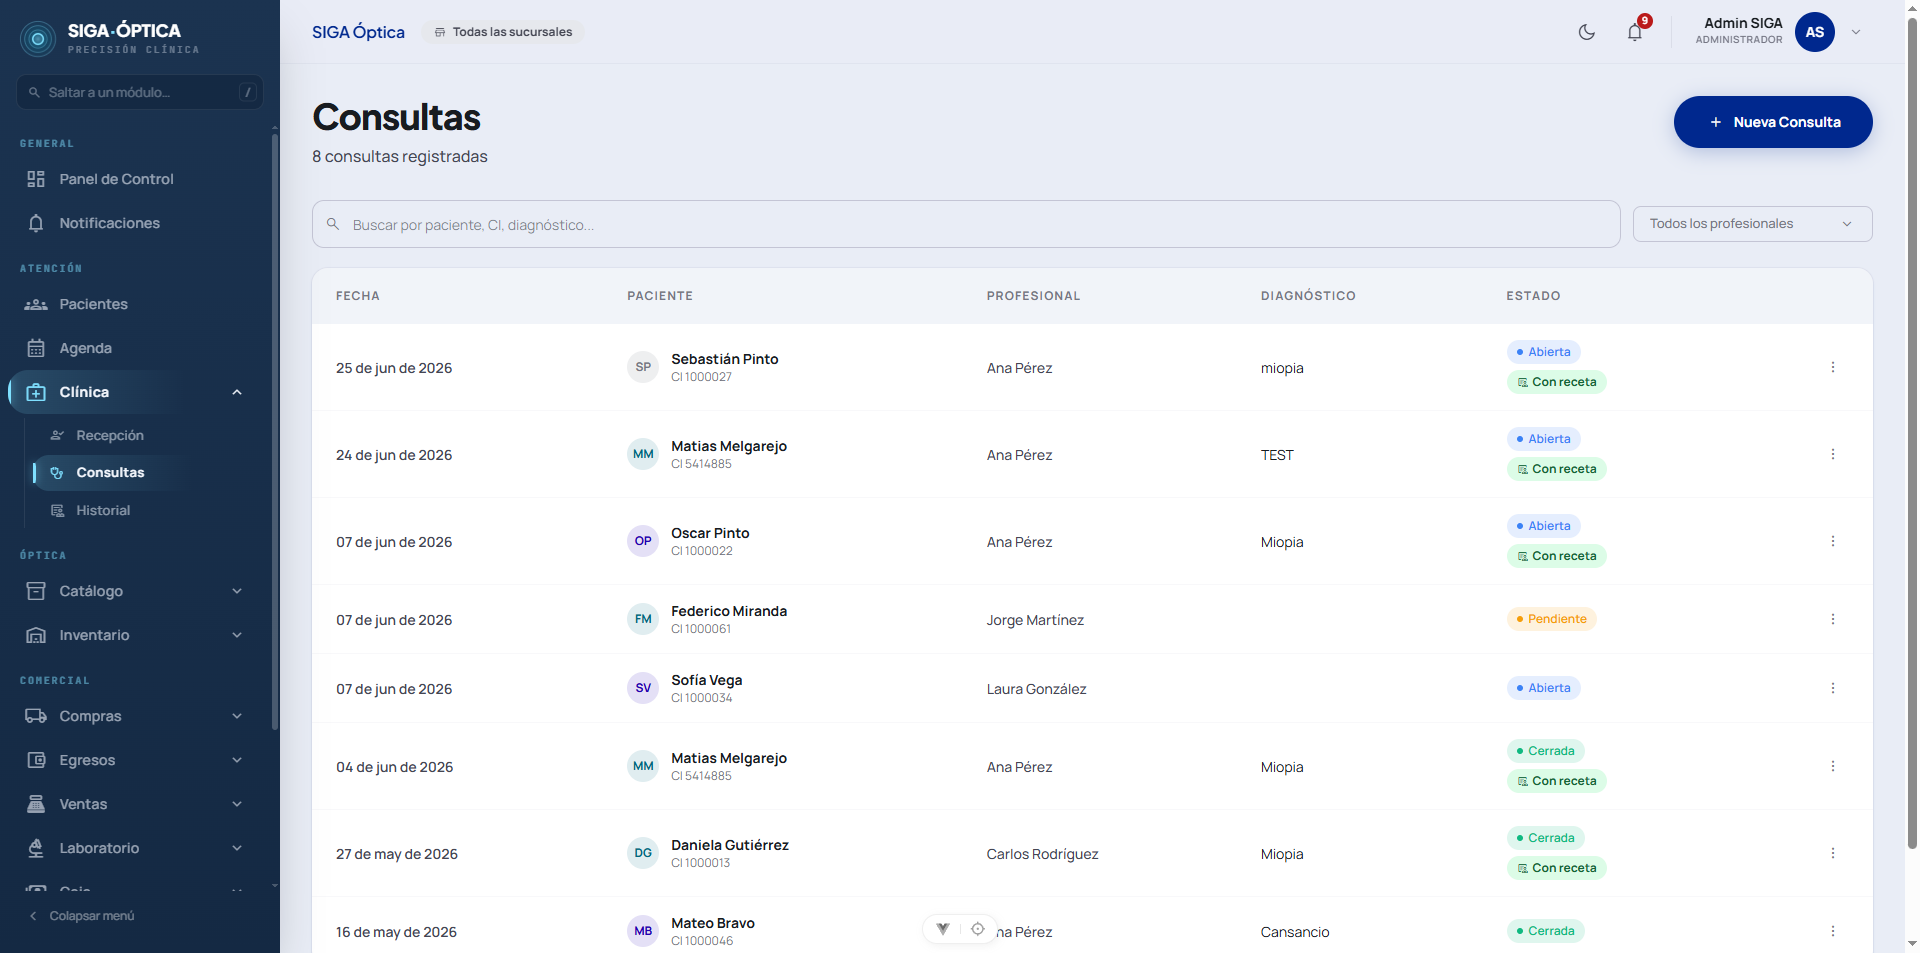
\includegraphics[width=0.95\textwidth]{imagenes/mod05-clinica-consultas.png}
\caption{Listado de consultas clínicas, con paciente, profesional, diagnóstico y estado.}
\label{fig:mod05-clinica}
\end{figure}

\section{Estado}
\label{sec:clinica-estado}

\Implementado\ y verificado end-to-end (self-booking del paciente, portal, PDF, receta externa).
